\documentclass[12pt,a4paper]{article}
\usepackage[utf8]{inputenc}
\usepackage[T1]{fontenc}
\usepackage{amsmath}
\usepackage{amsfonts}
\usepackage{amssymb}
\usepackage{graphicx} % Required for inserting images
\usepackage{geometry}
\usepackage{hyperref}
\usepackage{float} % Required for precise figure placement [H]
\geometry{margin=1in}

\title{\textbf{Labwork 2: Linear Regression from Scratch}}
\author{Pham Quang Duong - 2540048}
\date{\today}

\begin{document}

\maketitle

\section{Algorithm Implementation}

\subsection{Initialization and Objective Function}
At first, we initialize random $w_0$, $w_1$, learning rate r and threshold t:
\begin{equation}
w_0 = 0, w1 = 1, r = 0,0001, t = 10
\end{equation}

To calculate a single loss value, we use the function:
\begin{equation}
f(w_1, w_0, x_i, y_i) = \frac{1}{2}(w_1 x_i + w_0 - y_i)^2
\end{equation}

The total loss $L$ for all data points with $N$ samples is:
\begin{equation}
L(w_1, w_0) = \frac{1}{N} \sum_{i=1}^{N} \frac{1}{2}(w_1 x_i + w_0 - y_i)^2
\end{equation}

\subsection{Gradient Descent Optimization}
The update rules for each iteration are as follows:
\begin{align}
w_0 &:= w_0 - r \cdot \frac{\partial L}{\partial w_0} \\
w_1 &:= w_1 - r \cdot \frac{\partial L}{\partial w_1}
\end{align}
where $r$ is the learning rate. The partial derivatives (gradients) are calculated as follows:
\begin{align}
\frac{\partial L}{\partial w_0} &= \frac{1}{N} \sum_{i=1}^{N} (w_1 x_i + w_0 - y_i) \\
\frac{\partial L}{\partial w_1} &= \frac{1}{N} \sum_{i=1}^{N} x_i (w_1 x_i + w_0 - y_i)
\end{align}

\section{Visualization}
\begin{figure}[H]
    \centering
    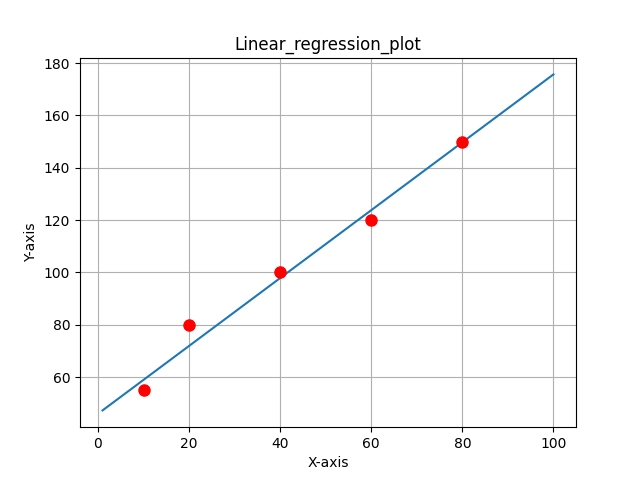
\includegraphics[width=0.8\textwidth]{Linear_regression_plot.png}
    \caption{Data and Regression Line.}
    \label{fig:regression_plot}
\end{figure}


\section{Analysis of Learning Rate ($r$)}
The learning rate is the most critical hyperparameter in this implementation:
\begin{itemize}
    \item \textbf{Small learning rate:} The algorithm takes very small steps. Although stable, it converges very slowly and requires a massive number of iterations to find the minimum value.
    \item \textbf{Optimal learning rate (Good):} The algorithm works efficiently. It moves towards the minimum point steadily and converges to the correct parameters in a reasonable number of iterations.
    \item \textbf{Large learning rate:} The algorithm takes steps that are too large. It may overshoot (jump over) the minimum point, causing the loss value to oscillate rather than strictly decrease.
    \item \textbf{Very large learning rate:} The algorithm completely fails to converge. The loss diverges because the updates move the weights further away from the minimum in every step.
\end{itemize}

\end{document}